\documentclass[letterpaper, 11pt]{article}
\usepackage[utf8]{inputenc}
\usepackage[letterpaper, portrait, margin=1in]{geometry}
\usepackage{pgfplots}
\pgfplotsset{width=10cm,compat=1.9}
\usepackage{hyperref}
\usepackage{textcomp}
\usepackage{siunitx}
\usepackage{amsmath}
\usepackage{cancel}
\usepackage{tikz}
\usepackage{everysel}
\usepackage{ragged2e}
\usepackage{mathdots}
\usepackage{yhmath}
\usepackage{color}
\usepackage{array}
\usepackage{multirow}
\usepackage{amssymb}
\usepackage{gensymb}
\usepackage{tabularx}
\usepackage{booktabs}
\usepackage{listings}
\usepackage{xcolor}
\usepackage{enumitem}
\usetikzlibrary{fadings}
\usetikzlibrary{patterns}
\usetikzlibrary{shadows.blur}
\hypersetup{
    colorlinks=true,
    linkcolor=black,
    filecolor=black,      
    urlcolor=blue,
}

\definecolor{codegreen}{rgb}{0,0.6,0}
\definecolor{codegray}{rgb}{0.5,0.5,0.5}
\definecolor{codepurple}{rgb}{0.58,0,0.82}
\definecolor{backcolour}{rgb}{0.95,0.95,0.92}

\lstdefinestyle{mystyle}{
    backgroundcolor=\color{backcolour},   
    commentstyle=\color{codegreen},
    keywordstyle=\color{magenta},
    numberstyle=\tiny\color{codegray},
    stringstyle=\color{codepurple},
    basicstyle=\ttfamily\footnotesize,
    breakatwhitespace=false,         
    breaklines=true,                 
    captionpos=b,                    
    keepspaces=true,                 
    numbers=left,                    
    numbersep=5pt,                  
    showspaces=false,                
    showstringspaces=false,
    showtabs=false,                  
    tabsize=2
}

\lstset{style=mystyle}

\title{COMSC-200 \\ Lab 8}
\author{Ryan Jacoby}
\date{1 November 2020}
\begin{document}

\maketitle

\section{Max Priority Queue}

\begin{lstlisting}[language=c++, caption=main.cpp]
// Ryan Jacoby

#include <chrono>
#include <cstdlib>
#include <ctime>
#include <iostream>

using namespace std;

int get_left_child_index(int);
int get_right_child_index(int);
void fix_heap(int *, int, int);
void heap_sort(int *, int);
void print(int *, int);

int insert(int *, int, int);
int pop(int *, int);

int main() {
    const int CAPACITY = 100;
    int nums[CAPACITY] = {8, 17, 4, 99, 3, 6, 88, 34, 65};
    int size = 9;

    heap_sort(nums, size);
    print(nums, size);

    insert(nums, 5, size);
    size++;
    print(nums, size);

    pop(nums, size);
    size--;
    print(nums, size);
    return 0;
}

int insert(int a[], int n, int last_index) {
    a[last_index] = n;
    heap_sort(a, last_index + 1);
    
    return 0;
}

int pop(int a[], int last_index) {
    int ret = a[0];
    a[0] = a[last_index - 1];
    heap_sort(a, last_index - 1);

    return ret;
}

int get_left_child_index(int index) {
    return 2 * index + 1;
}

int get_right_child_index(int index) {
    return 2 * index + 2;
}

void fix_heap(int a[], int root_index, int last_index) {
    int root_value = a[root_index];

    int index = root_index;
    bool done = false;
    while (!done) {
        int child_index = get_left_child_index(index);
        if (child_index <= last_index) {
            int right_child_index = get_right_child_index(index);
            if (right_child_index <= last_index && a[child_index] > a[right_child_index]) {
                child_index = right_child_index;
            }

            if (root_value > a[child_index]) {
                a[index] = a[child_index];
                index = child_index;
            } else {
                done = true;
            }
        } else {
            done = true;
        }
    }

    a[index] = root_value;
}

void heap_sort(int a[], int size) {
    int n = size - 1;
    for (int i = (n - 1) / 2; i >= 0; i--) {
        fix_heap(a, i, n);
    }
    
    while (n > 0) {
        // Swap root with the last element
        int temp = a[0];
        a[0] = a[n];
        a[n] = temp;
        n--;
        fix_heap(a, 0, n);
    }
}

void print(int a[], int size) {
    for (int i = 0; i < size; i++) {
        cout << a[i] << " ";
    }

    cout << endl;
}
\end{lstlisting}

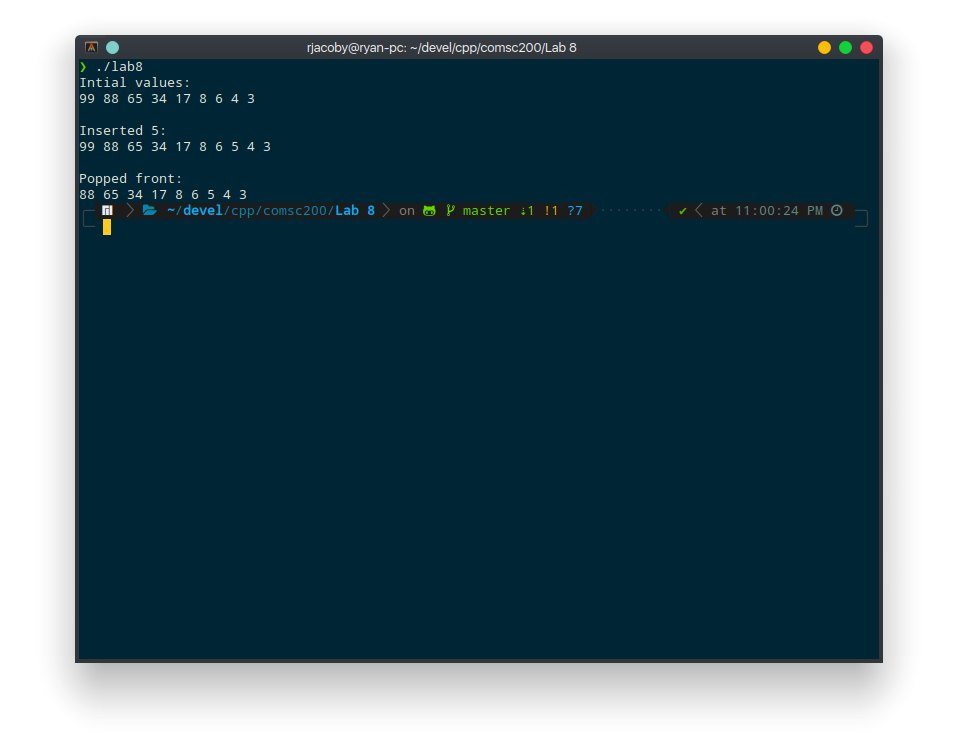
\includegraphics[scale=0.5]{max_pq.png}

\section{Heap Sort Process}

\includegraphics[]{heap_sort_diagram.png}

\section{Heap Sort}
Main function only, the rest of \textit{main.cpp} is unchanged.
\begin{lstlisting}[language=c++, caption=main]
int main() {
    const int CAPACITY = 100;
    int nums[CAPACITY] = {8, 17, 4, 99, 3, 6, 88, 34, 65};
    int size = 9;

    cout << "Unsorted:\n";
    print(nums, size);

    heap_sort(nums, size);

    cout << "\nSorted:\n";
    print(nums, size);
}
\end{lstlisting}

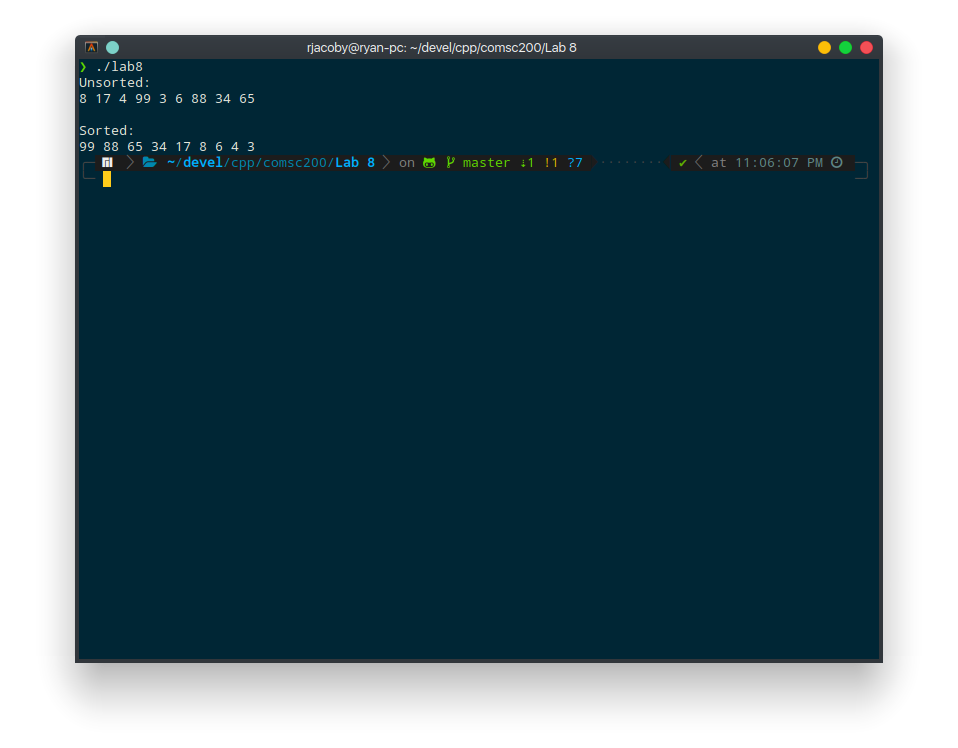
\includegraphics[scale=0.5]{heap_sort.png}

\section{Timed Heap Sort}
Main function only, the rest of \textit{main.cpp} is unchanged.
\begin{lstlisting}[language=c++, caption=main]
int main() {
    const int CAPACITY = 80000;
    int nums[CAPACITY];
    
    srand(time(NULL));
    for(int i = 0; i < CAPACITY; i++) {
        nums[i] = rand() % 100000 + 1;
    }

    cout << "Starting sort\n";
    auto start = chrono::high_resolution_clock::now();
    heap_sort(nums, CAPACITY);
    auto stop = chrono::high_resolution_clock::now();
    cout << "Sort complete\n\n";

    cout << "Sorted 80,000 integers in " << chrono::duration_cast<chrono::microseconds>(stop - start).count() << " microseconds\n";
}
\end{lstlisting}

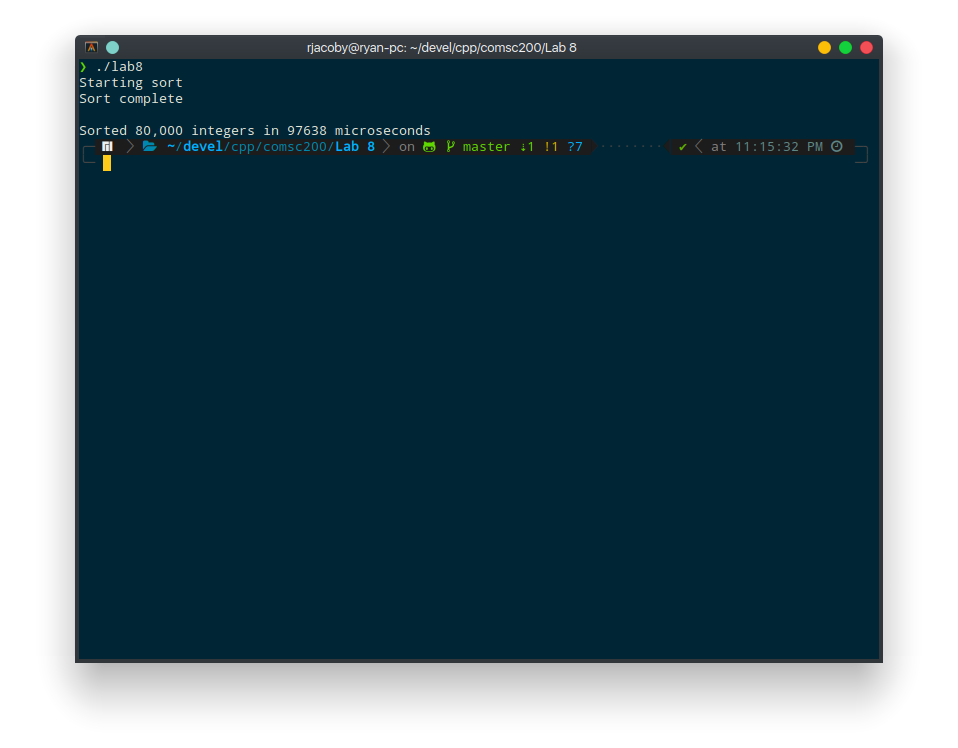
\includegraphics[scale=0.5]{heap_sort_timed.png}

\section{Float list}

\begin{lstlisting}[language=c++, caption=main.cpp]
// Ryan Jacoby

#include <chrono>
#include <cstdlib>
#include <ctime>
#include <iostream>

using namespace std;

int get_left_child_index(int);
int get_right_child_index(int);
void fix_heap(float *, int, int);
void heap_sort(float *, int);
void print(float *, int);

int insert(float *, float, int);
float pop(float *, int);

int main() {
    const int CAPACITY = 11;
    float nums[] = {0.6330566908, 0.1731436152, 0.8442427527, 0.3221575495, 0.5691910549, 0.9671822944, 0.5137396134, 
                    0.9039223096, 0.3170868986, 0.6026910402, 0.7127957556, 0.4026746783, 0.2412247231, 0.3896053414, 
                    0.8562880630, 0.6660960407, 0.0229718508, 0.5726884174, 0.1794473917, 0.9785428143, 0.9591225444, 
                    0.5237329453, 0.0731850322, 0.1319161876, 0.6595271659, 0.9627794760, 0.6963940613, 0.9510133140, 
                    0.0131817042, 0.8065370645};
    float a[CAPACITY];
    int size = 0;

    for(float f : nums) {
        if(size < CAPACITY) {
            insert(a, f, size);
            size++;
        } else {
            pop(a, size);
            size--;
            insert(a, f, size);
            size++;
        }
    }

    cout << "The 10 biggest floats in the test array are:\n";

    print(a, size);
}

int insert(float a[], float n, int last_index) {
    a[last_index] = n;
    heap_sort(a, last_index + 1);
    
    return 0;
}

float pop(float a[], int last_index) {
    int ret = a[0];
    a[0] = a[last_index - 1];
    heap_sort(a, last_index - 1);

    return ret;
}

int get_left_child_index(int index) {
    return 2 * index + 1;
}

int get_right_child_index(int index) {
    return 2 * index + 2;
}

void fix_heap(float a[], int root_index, int last_index) {
    float root_value = a[root_index];

    int index = root_index;
    bool done = false;
    while (!done) {
        int child_index = get_left_child_index(index);
        if (child_index <= last_index) {
            int right_child_index = get_right_child_index(index);
            if (right_child_index <= last_index && a[child_index] < a[right_child_index]) {
                child_index = right_child_index;
            }

            if (root_value > a[child_index]) {
                a[index] = a[child_index];
                index = child_index;
            } else {
                done = true;
            }
        } else {
            done = true;
        }
    }

    a[index] = root_value;
}

void heap_sort(float a[], int size) {
    int n = size - 1;
    for (int i = (n - 1) / 2; i >= 0; i--) {
        fix_heap(a, i, n);
    }
    
    while (n > 0) {
        float temp = a[0];
        a[0] = a[n];
        a[n] = temp;
        n--;
        fix_heap(a, 0, n);
    }
}

void print(float a[], int size) {
    for (int i = 0; i < size; i++) {
        cout << a[i] << " ";
    }

    cout << endl;
}    
\end{lstlisting}

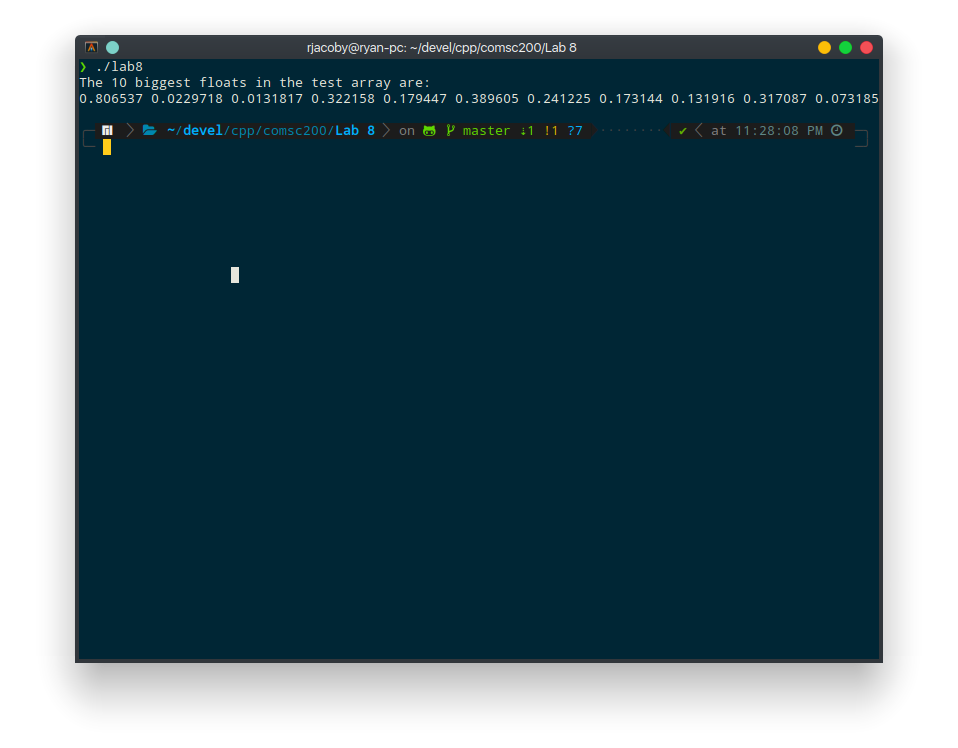
\includegraphics[scale=0.5]{floats.png}

\end{document}
